\documentclass[openany]{book}
\usepackage{lmodern}
\usepackage{amssymb,amsmath}
\usepackage{ifxetex,ifluatex}
\usepackage{fixltx2e} % provides \textsubscript
\ifnum 0\ifxetex 1\fi\ifluatex 1\fi=0 % if pdftex
  \usepackage[T1]{fontenc}
  \usepackage[utf8]{inputenc}
\else % if luatex or xelatex
  \ifxetex
    \usepackage{mathspec}
  \else
    \usepackage{fontspec}
  \fi
  \defaultfontfeatures{Ligatures=TeX,Scale=MatchLowercase}
\fi
% use upquote if available, for straight quotes in verbatim environments
\IfFileExists{upquote.sty}{\usepackage{upquote}}{}
% use microtype if available
\IfFileExists{microtype.sty}{%
\usepackage{microtype}
\UseMicrotypeSet[protrusion]{basicmath} % disable protrusion for tt fonts
}{}
\usepackage[margin=1in]{geometry}
\usepackage{hyperref}
\hypersetup{unicode=true,
            pdftitle={Systems Pathology: Muscle System},
            pdfauthor={Russell Fraser},
            pdfborder={0 0 0},
            breaklinks=true}
\urlstyle{same}  % don't use monospace font for urls
\usepackage{natbib}
\bibliographystyle{apalike}
\usepackage{longtable,booktabs}
\usepackage{graphicx,grffile}
\makeatletter
\def\maxwidth{\ifdim\Gin@nat@width>\linewidth\linewidth\else\Gin@nat@width\fi}
\def\maxheight{\ifdim\Gin@nat@height>\textheight\textheight\else\Gin@nat@height\fi}
\makeatother
% Scale images if necessary, so that they will not overflow the page
% margins by default, and it is still possible to overwrite the defaults
% using explicit options in \includegraphics[width, height, ...]{}
\setkeys{Gin}{width=\maxwidth,height=\maxheight,keepaspectratio}
\IfFileExists{parskip.sty}{%
\usepackage{parskip}
}{% else
\setlength{\parindent}{0pt}
\setlength{\parskip}{6pt plus 2pt minus 1pt}
}
\setlength{\emergencystretch}{3em}  % prevent overfull lines
\providecommand{\tightlist}{%
  \setlength{\itemsep}{0pt}\setlength{\parskip}{0pt}}
\setcounter{secnumdepth}{5}
% Redefines (sub)paragraphs to behave more like sections
\ifx\paragraph\undefined\else
\let\oldparagraph\paragraph
\renewcommand{\paragraph}[1]{\oldparagraph{#1}\mbox{}}
\fi
\ifx\subparagraph\undefined\else
\let\oldsubparagraph\subparagraph
\renewcommand{\subparagraph}[1]{\oldsubparagraph{#1}\mbox{}}
\fi

%%% Use protect on footnotes to avoid problems with footnotes in titles
\let\rmarkdownfootnote\footnote%
\def\footnote{\protect\rmarkdownfootnote}

%%% Change title format to be more compact
\usepackage{titling}

% Create subtitle command for use in maketitle
\newcommand{\subtitle}[1]{
  \posttitle{
    \begin{center}\large#1\end{center}
    }
}

\setlength{\droptitle}{-2em}

  \title{Systems Pathology: Muscle System}
    \pretitle{\vspace{\droptitle}\centering\huge}
  \posttitle{\par}
    \author{Russell Fraser}
    \preauthor{\centering\large\emph}
  \postauthor{\par}
      \predate{\centering\large\emph}
  \postdate{\par}
    \date{2019-02-20}

\usepackage{booktabs}

\begin{document}
\maketitle

{
\setcounter{tocdepth}{1}
\tableofcontents
}
\chapter*{About}\label{about}
\addcontentsline{toc}{chapter}{About}

These represent the course notes for the skeletal muscle system for VETM
2220. They are broken down into several sections based on disease
process.

\subsection*{Contact me}\label{contact-me}
\addcontentsline{toc}{subsection}{Contact me}

Please don't hesitate to get in touch if you have any questions.

\begin{itemize}
\tightlist
\item
  Phone: 902-620-5183
\item
  E-mail: \href{mailto:rufraser@upei.ca}{\nolinkurl{rufraser@upei.ca}}
\item
  Office: 414N
\end{itemize}

\chapter{Introduction}\label{intro}

\section{The anatomy of muscle}\label{the-anatomy-of-muscle}

The basic structural unit of muscle is the \textbf{myofiber}, which
represents a single, long, tubular cell (Figure
\ref{fig:muscle-structure}). Within each myofiber are many tightly
packed \textbf{myofibrils}, which are composed of actin and myosin
filaments, and which form the contractile machinery of the muscle. It is
the arrangment of myofibrils that form the striated appearance of
skeletal muscle that can be appreciated under light microscopy (Figure
\ref{fig:muscle-histo}). The cytoplasm of a myofiber is known as the
\textbf{sarcoplasm}, while the cell membrane is called the
\textbf{sarcolemma}. Each myofiber is surrounded by a small amount of
connective tissue called the \textbf{endomysium}. Multiple myofibers
form a \textbf{fasicle} that is surrounded by another layer of
connective tissue, the \textbf{perimysium}. Finally, multiple fasicles
group together to form a muscle.

\begin{figure}

{\centering 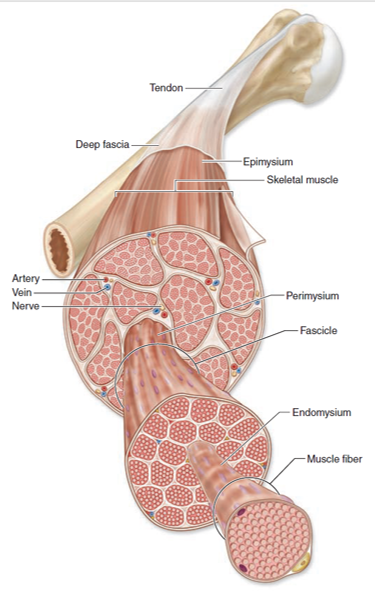
\includegraphics[width=0.6\linewidth]{images/muscle_structure} 

}

\caption{Structure and anatomy of muscle}\label{fig:muscle-structure}
\end{figure}

\begin{figure}

{\centering 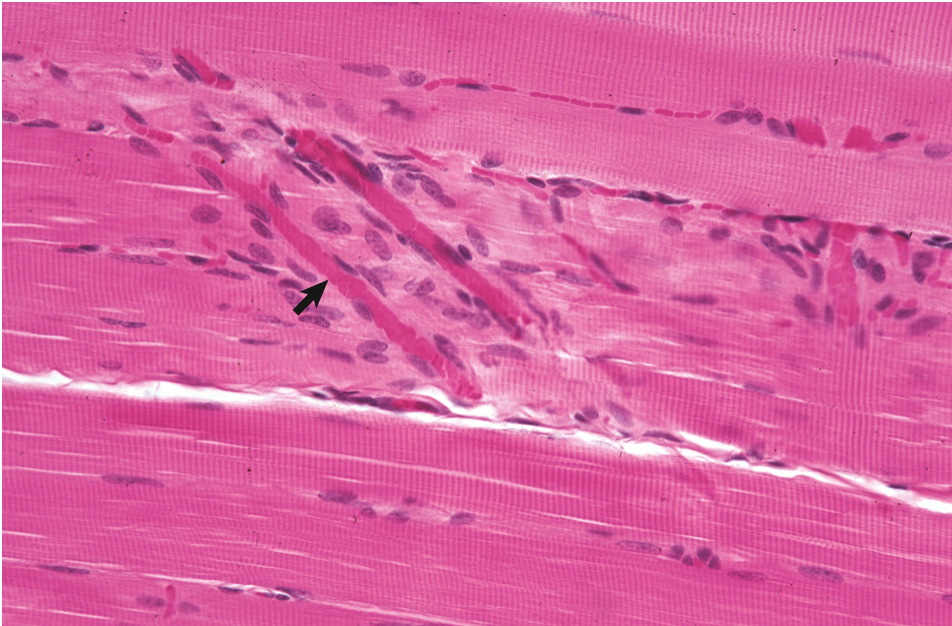
\includegraphics[width=0.8\linewidth]{images/muscle_histo} 

}

\caption{Normal skeletal muscle demonstrating striations. The arrow indicates a small capillary.}\label{fig:muscle-histo}
\end{figure}

Skeletal muscle is characteristically multinucleated: each myofiber has
100s of nuclei scattered along its length, almost always found along the
periphery of the cell. Each nucleus within a myofiber controls a
specific portion of the myofiber, and each nucleus acts independently.
Nuclei within muscle fibers are \emph{terminally differentiated},
meaning they can no longer divide, thus limiting the capacity for
regeneration. On the other hand, having multiple nuclei within a cell
provides a distinct benefit: localized damage, affecting a small number
of nuclei, will not necessarily kill the entire cell, giving the
myofiber an opportunity to regenerate. We will discuss muscle
regeneration in more detail in the section on
\protect\hyperlink{necrosis-and-regeneration}{Necrosis and
regeneration}.

Closely associated with individual myofibers are \textbf{satellite
cells}. The nuclei of satellite cells are indistinguishable from
myofiber nuclei under light microscopy. Satellite cells are a type of
stem cell, and are important in muscle regeneration and repair.

Myofibers can be subclassified based on certain properties that reflect
their function. The classification is based on three physiologic
properties:

\begin{enumerate}
\def\labelenumi{\arabic{enumi}.}
\tightlist
\item
  Rate of contraction (fast vs.~slow)
\item
  Rate of fatigue (fast vs.~slow)
\item
  Type of metabolism (oxidative, glycolytic, or mixed)
\end{enumerate}

Taking these characteristics into consideration leads to three subtypes:
Type 1, Type 2a, and Type 2b (Table \ref{tab:muscle-type}). Note that
muscles are rarely, if ever, composed of a single subtype: they are a
mixture of the different subtypes, though one type often predominates.

\begin{table}[t]

\caption{\label{tab:muscle-type}Properties of different myofiber types}
\centering
\begin{tabular}{l|l|l|l}
\hline
Fiber.type & Physiologic.characteristics & Morphologic.characteristics & Examples\\
\hline
Type 1 & slow twitch, fatigue resistant, oxidative, aerobic, 'red' & High mitochondrial and fat content, low glycogen & Muscles involved in prolonged activity, e.g. postural muscles, diaphragm\\
\hline
Type 2a & Fast twitch, oxidative, glycolytic, fatigue resistant & Intermediate mitochondria, fat, and glycogen content & \\
\hline
Type 2b & Fast twitch, fatigue sensitive, glycolytic, 'white' & Low mitochondrial and fat content, high glycogen & Muscles involved in athletic acitivty, e.g. sprinting\\
\hline
\end{tabular}
\end{table}

\section{The function of muscle}\label{the-function-of-muscle}

The contraction of muscle is a complex, orchestrated process in which
myofilaments (the components of myofibrils) undergo a conformational
change that results. The contraction of muscle is initiated at the
\textbf{motor end plate} by the release of acetylcholine from a motor
neuron into the neuromuscular junction. This depolarizes the myofiber,
resulting in the release of \textbf{calcium} from the sarcoplasmic
reticulum. It is the binding of calcium to the myofilament tropononin
that results in the contraction of the sarcomere. Importantly, calcium
must be pumped back into the sarcoplasmic reticulum in an ATP-dependent
process. Once this occurs, the muscle enters into a relaxed, resting
state.

\section{Response of muscle to
injury}\label{response-of-muscle-to-injury}

Skeletal muscle can undergo a fairly limited range of changes in
response to environmental and physiologic stimuli. Muscle can shrink
(atrophy), get bigger (hypertrophy), or die (necrosis). Under certain
circumstances, muscles that have been only mildly injured can
regenerate. The reaction of muscle to injury tends to proceed in a
fairly sterotypic fashion regardless of the inciting cause, making it
difficult to determine the underlying etiology from gross or
histopathological exmaination alone. Thus, \textbf{it is important to
provide a good clinical history} when submitting a case with suspected
muscle injury. Supplementary tests (special stains, culture, etc.) are
also often necessary to obtain a definitive diagnosis.

\subsection{Atrophy}\label{atrophy}

Atrophy simply refers to the reducing in volumne of muscle or myofiber,
and is usually reversible, provided the cause can be corrected.

\subsubsection{Denervation atrophy}\label{denervation-atrophy}

Denervation atrophy is caused by the loss of a nerve that innervates a
myofiber. It is rapid, severe, relatively common, and can result in the
loss of more than half of the affected muscle mass in a matter of weeks.
The maintenance of a normal myofiber diameter is reliant in part on an
intact associated nerve, which generates trophic factors. Loss of a
nerve leads to loss of the trophic factors, and results in atrophy.
Interestingly, it is not a factor of contractile activity: disorders
such as {[}Botulism{]} or {[}Tetanus{]} that affect the neuromuscular
junction do not lead to atrophy. Denervation atrophy tends to affect
affect both type 1 and 2 myofibers. Examples of disorders caused by
denervation atrophy include {[}Equine laryngeal hemiplegia
(``roaring''){]}, {[}``Sweeney''{]}, {[}Equine motor neuron disease{]},
{[}Equine protozoal myeloencephalitis{]}, and {[}Radial nerve
paralysis{]}.

\subsubsection{Disuse atrophy}\label{disuse-atrophy}

Decreased contractile activity of a muscle for any reason leads to
disuse atrophy. Common causes include lameness/pain or limb
immobilization (e.g.~cast), and it tends to occur more gradually then
denervation atrophy. Disuse atrophy preferentially leads to atrophy of
type 2 fibers, however, this is somewhat inconsistent, thus relying
solely on type 2 atrophy to distinguish this from denervation atrophy is
risky. Because the muscle fibers undergoing disuse atrophy are not being
used, there is no compensatory hyertrophy.

\subsubsection{Nutritional (malnutrition or cachexia)
atrophy}\label{nutritional-malnutrition-or-cachexia-atrophy}

Failure to supply enough dietary nutrients to maintain normal muscle
mass leads to nutritional atrophy. It is a gradual form of muscle loss
and tends to be generalized, though in the dog, loss of the temporal,
back, and thigh muscles are often prominent. Muscle proteins undergo
continuous turnover, and in states of starvation, can be used as a
source of nutrients. Cachectic animals with chronic illness or neoplasia
lose muscle mass due to increased circulating levels of \textbf{TNF}
(also known as ``cachectin''), which increases myofiber catabolism. Type
2 fibers are preferentially affected.

\subsubsection{Atrophy of endocrine
disease}\label{atrophy-of-endocrine-disease}

This is a relatively specific category of atrophy, most commonly noted
in dogs with hypothyroidism or hyperadrenocorticism. Type II fibers are
preferentially affected.

\subsection{Hypertrophy}\label{hypertrophy}

Hypertrophy refers to grossly enlarged muscles, or to histologically
enlarged myofibers. It does \emph{not} refer to an increase in number of
myofibers. It can be the result of physiologic stimulation or pathologic
processes. Physiologic hypertrophy is generally the result of increased
workload on the muscle. Pathologic hypertrophy occurs in response to a
number of conditions. Compensatory hypertrophy of unaffected myofibers
can occur in a background of neuropathic or myopathic atrophy.

\hypertarget{necrosis-and-regeneration}{\subsection{Necrosis and
regeneration}\label{necrosis-and-regeneration}}

Myofiber necrosis is a non-specific finding that can accompany a variety
of different diseases and conditions. Grossly, necrosis of muscle is
usually only appreciated in severe cases. Necrotic muscle is typically
pale to white, and may appear streaked and slightly gritty if
mineralization has occurred (for example, in {[}White muscle
disease{]})(Figure \ref{fig:heart-necrosis}). Necrotic muscle can
alternatively appear deeply red, if hemorrhage has occurred
concurrently.

\begin{figure}

{\centering 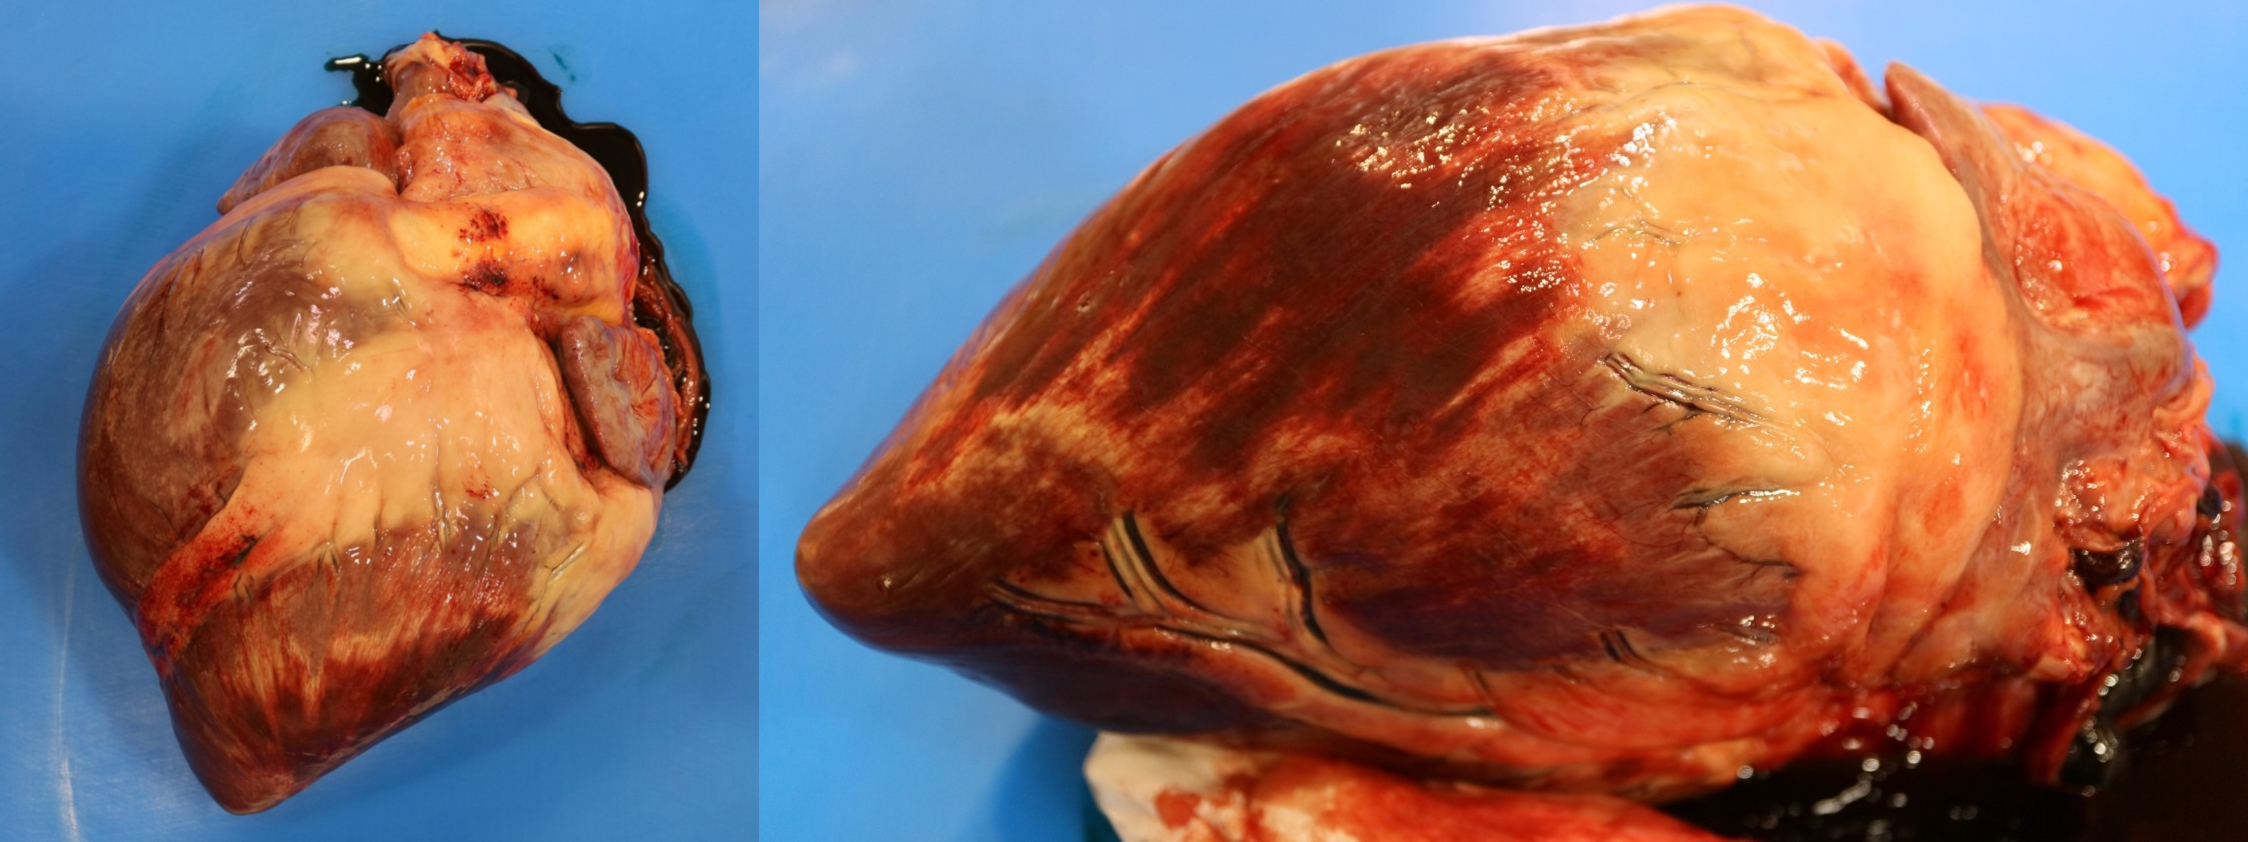
\includegraphics[width=0.6\linewidth]{images/heart-necrosis-comp} 

}

\caption{Necrosis of the myocardium. Pale white streaks bordered by hemorrhage are visible throughout the ventricle. Photo: C. Martin}\label{fig:heart-necrosis}
\end{figure}

The outcome of muscle necrosis is dependent on its severity. If the
basal lamina remains intact, and the damage only affects a small portion
of the myofiber, then muscle can regenerate. The basal lamina is a thin
layer of extracellular matrix that keeps satellite cells closely
associated to the myofiber, and just importantly, keeps fibroblasts out.
The steps in muscle regeneration are fairly straightforward:

\begin{enumerate}
\def\labelenumi{\arabic{enumi}.}
\tightlist
\item
  Segmental necrosis
\item
  Invasion of the sarcoplasm by circulating monocytes, which
  differentiate into macrophages.

  \begin{enumerate}
  \def\labelenumii{\roman{enumii})}
  \tightlist
  \item
    Macrophages phagocytose cellular debris, ``cleaning'' up the
    sarcoplasm.
  \end{enumerate}
\item
  Satellite cells enter the sarcoplasm and migrate towards the center of
  the of the myofiber.
\item
  Satellite cells divide and form a tube (``myotube'') which produces
  sarcoplasm.

  \begin{enumerate}
  \def\labelenumii{\roman{enumii})}
  \tightlist
  \item
    The myotube extends to the edges of the damaged myofiber.
  \item
    The myotube expands, though is still narrower than the unaffected
    myofiber.
  \item
    A row of nuclei appear in the center of the regenerating myofiber,
    and sarcomeres begin to form.
  \end{enumerate}
\end{enumerate}

Note that if the basal lamina has been destroyed, or if the damage
affects a large area, then healing occurs via fibrosis (scarring).
Although myofiber nuclei themselves cannot divide, recall that each
myofiber is accompanied by \textbf{satellite cells}, which can divide
and differentiate into myofibers.

Segmental necrosis and regeneration occur following a variety of
insults, most commonly metabolic, nutritional (e.g. {[}White muscle
disease{]}, toxic (e.g. {[}Ionophore toxicity{]})). Determining the
etiology of the damage can therefore be quite difficult. It is helpful
to observe the temporal pattern of the damage: are all muscle fibers at
the same stage of necrosis or regeneration, suggesting a single, massive
insult? Or is there a range of changes, with some fibers showing early
stages of necrosis, and others at the end of regeneration, which
suggests an on-going injury? These temporal changes are known as
\textbf{monophasic} (occuring at one point) or \textbf{polyphasic} (an
on-going proceess). These can be further classified by the commonly used
distribution modifiers: focal, locally extensive, multifocal, or
diffuse, to help narrrow down the etiology. For example, a focal,
monophasic injury is more likely to be traumatic in origin than
metabolic, while a multifocal, polyphasic injury could be due to the
on-going lack of a nutritional requirement, as seen in {[}White muscle
disease{]}.

\section{Gross evaluation of muscle}\label{gross-evaluation-of-muscle}

Although important, the gross examination of muscles during a necropsy
can be underwhelming, and if muscular disease is suspected, samples of
muscle should \emph{always} be submitted for histopathology. During a
gross examination of a carcass, muscles should be evaluated for changes
in size, texture, and colour. Muscles can be bigger (hypertrophied) or,
more commonly, smaller (atrophied), or normal. Difficulty in assessing
the normal size of muscles for different species and breeds can be aided
by comparing with normal animals, or, if unilateral disease is present,
with the contralateral side.

Changes in the colour of muscle are common, are often artifactual, and
are dependent on blood perfusion, age, and species. Possible colour
changes, along with potential causes, are listed below.

\begin{itemize}
\tightlist
\item
  Pale muscles:

  \begin{itemize}
  \tightlist
  \item
    Normal in young animals
  \item
    Common in anemic animals
  \item
    Can be due to necrosis (ischemic)
  \item
    Denervation
  \item
    If streaking observed, usually due to necrosis and mineralization.
  \end{itemize}
\item
  Dark red:

  \begin{itemize}
  \tightlist
  \item
    Congestion or hemorrhage
  \item
    Hemorrhagic necrosis
  \item
    Inflammation
  \item
    Hypostatic congestion (i.e.~blood pooling due to gravity, and
    artifact found in postmortem examinations)
  \end{itemize}
\item
  Green:

  \begin{itemize}
  \tightlist
  \item
    Putrefaction (rot)
  \item
    Eosinophilic inflammation (uncommon)
  \end{itemize}
\end{itemize}

The texture of diseased muscle can range from soft to hard
(mineralized). Soft muscle can be indicative of necrosis, or potentially
fat infiltration.

\section{Biopsy techniques}\label{biopsy-techniques}

As noted above, a biopsy of muscle should always accompany any suspected
muscular disease. Muscle is highly susceptible to artifact, but proper
preparation of the sample can help in ensuring a diagnostic sample.
Muscle retains the ability to contract after biopsy/death, and this
contraction can result in artifactual histological changes that mimic
true pathological changes. These changes, noted as \emph{contraction
band artifact}, can be prevented relatively easily: shortly after
removal, secure the muscle to a rigid surface prior to fixation. A
simple and manageable technique whether in the field or clinic is to
place a strip of muscle along a tongue depressor, and anchor it into
place using two needles (FIGURE XXX GET PICTURE), prior to placing the
sample in formalin. As a general rule, a muscle biopsy should not exceed
\textasciitilde{} 1 cm in diameter (with myofibers running lengthwise).

\chapter{Congenital and inherited
myopathies}\label{congenital-and-inherited-myopathies}

\chapter{Circulatory disturbances}\label{circulatory-disturbances}

We describe our methods in this chapter.

\chapter{Physical injuries}\label{physical-injuries}

\chapter{Toxic myopathies}\label{toxic-myopathies}

We have finished a nice book.

\chapter{Degenerative/necrotizing
myopathies}\label{degenerativenecrotizing-myopathies}

We have finished a nice book.

\chapter{Myopathies associated with endocrine
disorders}\label{myopathies-associated-with-endocrine-disorders}

We have finished a nice book.

\chapter{Myopathies associated with serum electrolyte
imbalance}\label{myopathies-associated-with-serum-electrolyte-imbalance}

We have finished a nice book.

\chapter{Immune-mediate myopathies}\label{immune-mediate-myopathies}

\section{Masticatory myositis}\label{masticatory-myositis}

\section{Acquired myasthenia gravis}\label{acquired-myasthenia-gravis}

We have finished a nice book.

\chapter{Infectious myositis}\label{infectious-myositis}

\section{Clostridial myositis}\label{clostridial-myositis}

\section{}\label{section}

\chapter{Parasitic myositis}\label{parasitic-myositis}

\section{Sarcocystosis}\label{sarcocystosis}

\section{Neospora caninum and Toxoplasma
gondii}\label{neospora-caninum-and-toxoplasma-gondii}

\section{}\label{section-1}

\chapter{Neoplasms of muscle}\label{neoplasms-of-muscle}

Primary neoplasms of the striated muscle are rare in veterinary species.
Although usually found in muscle, they can arise in unexpected locations
devoid of striated muscle, such as the bladder.

\section{Rhabdomyoma}\label{rhabdomyoma}

As it's name suggests, a rhabdomyoma is a benign tumour of striated
muscle. It is seen most frequently in the hearts of pigs, particularly
the red wattle breed and are typically incidental findings. They often
present grossly as circumscribed, smooth-surfaced, nodular masses
embedded in the myocardium. A similar neoplasm occasionally arises on
the larynx of dogs. Laryngeal rhadomyomas may cause respiratory
difficulty or altered bark. They are typically minimally invasive and
tend not to metastasize.

\section{Rhabdomyosarcoma}\label{rhabdomyosarcoma}

These are the malignant counterparts to rhadomyomas. They are most
common in the dog. Counterintuitively, they occur more frequently at
sites that normally lack skeletal muscle versus those that don't. There
are a variety of subtypes, however, whether there is any prognostic
significance to differentiating them is uncertain. They all tend to be
locally invasive and metastatic. Prognosis is poor for all subtypes.
Grossly, the tumours appear as pale, white to tan, firm masses, often
with areas of necrosis. The botryoid (``cluster of grapes'') subtype
occurs in the bladder as a polypoid mass. The histologic appearance of
these tumours is quite variable, though occasionally elongated, variably
striated, myotube-like cells known as ``strap cells'' are present, which
is suggestive of rhadomyosarcoma. Immunohistochemistry is usually
required to definitively diagnose these tumours.

\section{Tumours of the s}\label{tumours-of-the-s}

The supporting mesenchyme of muscle can occasionally produce a (usually)
malignant neoplasm. Granular cell tumours occur in the tongue of dogs
and cats. They are composed of densely packed round cells with PAS
positive granules. Hemangiosarcomas can arise in the muscles of dogs and
horses, and aspiration of these large, intramuscular masses typically
only reveals hemorrhage. Like their splenic cousins, they metastasize
frequently.

\section{Secondary tumours}\label{secondary-tumours}

Muscles are occasionally infiltrated by local neoplasms. Infiltrative
lipomas are characterized by relatively well differentiated adipocytes
crawling and invading through myofibers. They are highly invasive and
require excision. Other neoplasms, such as subcutaneous mast cell
tumours, lymphoma, hemangiosarcomas, and soft tissue sarcomas can invade
into muscle. Metastasis to muscle is uncommon but does occur.

\bibliography{book.bib,packages.bib}


\end{document}
